% !TeX root = 00_Vorlage.tex
% !TeX spellcheck = de_DE
\section{Diskussion und Schlussfolgerung}
\label{chap:schlussfolgerung}

In diesem Kapitel werden die Beobachtungen und Berechnungen der Versuche diskutiert, mit besonderem Augenmerk auf das Kernthema diesen Berichtes, das vorgeschlagene Modell.

In \autoref{table:Zusammenfassung} wurden die gemessenen und theoretisch bestimmten Werte eingetragen.  Da das Modell auf dem experimentell bestimmten Wert für \( k_1 \) basiert wird kein theoretisch bestimmter Wert angegeben, da das ein Zirkelschluss wäre, jedoch den Anschein hätte, es würde unser Modell unterstützen.

\begin{center}
	\captionof{table}[Zusammenfassung des Versuchs]{Gegenüberstellung der experimentell bestimmten und theoretisch berechneten Werte für $k_i$}
	\begin{tabular}{@{\extracolsep{5mm}} 
			r
			S[table-format=2.2(2)]
			S[table-format=2.1(1)]
			S[table-format=2.1(1)]
		}
		\toprule
		\makecell[t]{}
		&   {\makecell[t]{\( k_1 \unit{(N/m)} \)}}
		&   {\makecell[t]{\( k_2 \unit{(N/m)}\)}}
		&   {\makecell[t]{\( k_3 \unit{(N/m)}\)}}\\
		\midrule
		Experimenteller Wert & 14.00(17) &  27.5(5)  & 41.2(8)\\
		Theoretischer Wert & & 28.0(2) & 42.0(5)\\
		\bottomrule
	\end{tabular}
	\label{table:Zusammenfassung}
\end{center}

Vergleicht man nun die aus vorigen Kapiteln berechneten Werte für $k_i$, erkennt man, dass die experimentell bestimmten Werte für $k_i$ mit denen von uns entwickelten Modell:
\begin{align}
	k_{\text{ges}} = \sum_{i=1}^{N} k_i &&\text{bzw. bei identischen Federn} && k_{\text{ges}} = N*k
\end{align} 
im Rahmen der Unsicherheit übereinstimmen.

In \autoref{fig:Diskusisons} wurden in der oberen Abbildung die Federkonstante auf die Anzahl der Federn aufgetragen. In rot ist das lineare Modell (basierend auf \( k_1 \)) zu als Vergleich zu sehen. Die Werte sind weniger als eine Standardabweichung vom Modell entfernt und lassen unterstützen es daher. Dies wird noch deutlicher wenn man die Federkonstante durch die Anzahl der Federn teilt (Siehe untere Graphik), um aus einer linearen Zunahme eine Konstante zu machen. Die Werte für \( k_2 \) und \( k_3 \) liegen mitsamt Fehler innerhalb des \( 1\sigma- \)Bandes des Modells.

\begin{figure}[H]
	\centering
	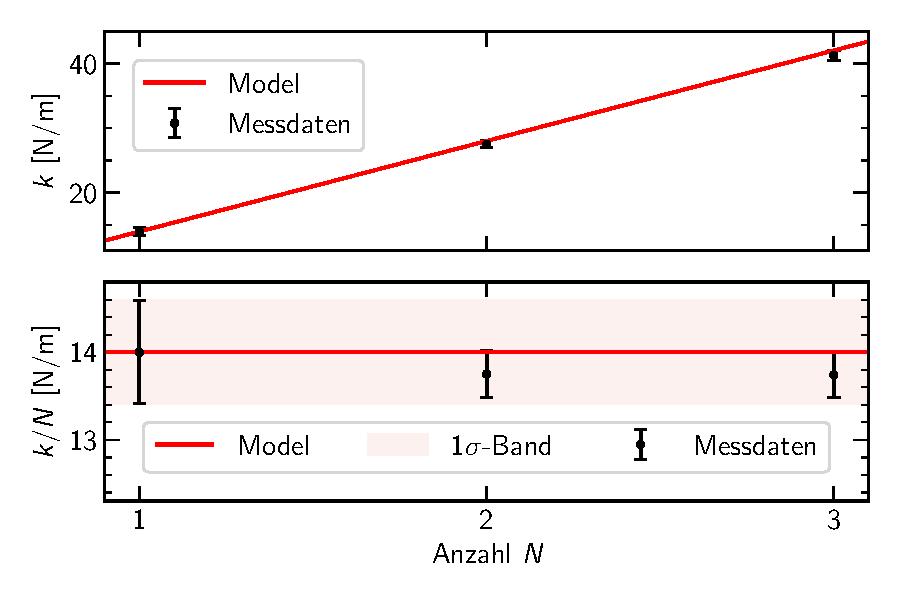
\includegraphics[width=\textwidth]{Diskussion.pdf}
	\caption[Vergleich der Federkonstanten als normalisierte Gaußkurven]{Oben wurde die gemessene Federkonstante auf die Anzahl der Federn aufgetragen. Unten wurde die Federkonstante durch die Anzahl der Federn geteilt. In beiden Graphiken ist in rot das Modell aufgetragen.}
	\label{fig:Diskusisons}
\end{figure}

Die hier präsentierten Resultate sind konsistent und unterstützen das Modell, die Fehler jedoch sind recht groß, da die statistische Unsicherheit alleine circa \( 2 \% \) des Nennwertes beträgt. Hinzu kommen noch systematische Abweichungen, die in diesem Bericht nicht im Detail diskutiert wurden, sich aber zum Beispiel durch die Verwendung eines (gering) elastischen Stückes Hartpapier eingeschlichen haben. Um den statistischen Fehler zu reduzieren, müsste man die Masse genauer bestimmen, am Besten über eine geeichte Waage, und die Schwingungen länger aufzeichnen, da die Unsicherheit im Fit so minimiert werden kann.

Erwähnenswert ist auch, dass hier zwar ein allgemein gültiges Modell für die Kombination von parallelen Federn präsentiert wurde, es jedoch nur auf einen Spezialfall geprüft wurde, nämlich der, wo alle Federn gleich sind. Man müsste weitere Versuche mit Federn mit unterschiedlichen Federkonstanten oder sogar Federn unterschiedlicher Natur (Metallfeder, Dämpfer) durchführten, um die Gültigkeit dieses Modells auszuweiten. 


